In this chapter I will give an overview of how this audio codec will be designed, and explaining the various decisions I made along the way.

I have decided to call this new codec \emph{ANMF} (stands for Audio-NMF), using files with the extension \emph{.anmfx}, where \emph{x} represents the compression method. It will be implemented as a command line utility.

There are currently three different ANMF formats that you can choose from, and their main difference is which audio representation is being compressed by NMF. They are as follows:

\begin{description}
	\item[ANMF-RAW] denoted by \emph{r}, compresses the signal in PCM form (time domain)
	\item[ANMF-MDCT] denoted by \emph{m}, compresses the signal transformed with MDCT (frequency domain)
	\item[ANMF-STFT] denoted by \emph{s}, compresses the signal transformed with STFT (frequency domain)
\end{description}

\section{WAVE file}
WAVE, WAV or Waveform audio is a file format for storing digitized audio, created as a joint design by the Microsoft Corporation and the IBM Corporation. They are built on top of the chunk-based RIFF format. For details on the specific structure of a WAVE file please refer to \cite{sapp_pcm}.

It stores raw uncompressed audio samples in PCM format along with some metadata and will serve as both the standard input and output to the ANMF codec. Most commonly used formats can be converted to and from WAV as well and thus it will serve as a good baseline.

Samples in this format can be represented by different datatypes, I chose 16-bit signed integers, i.e. each sample's amplitude is represented by a whole number between $-32768$ and $32767$. The sample rate can vary, but a good standard value the experiments will use is $44.1$ kHz, which corresponds to audio CD quality.

\section {ANMF File structure}
The base container for the compressed ANMF file is the same no matter which encoding method you use. The bytes are saved in little endian byte order.

Please refer to Table \ref{tab:anmf_file} and each encoding method's table for the specific file structure. The first eleven bytes are mostly set in stone other than the method specification, but after that it varies greatly.

\begin{table}[htbp]\caption{ANMF file structure}
	\label{tab:anmf_file}
	\centering
	\begin{tabular}{|c|c|l|}
		\hline
		Bytes & Data type & Description \\ \hline
		0-3 & char[] & identifier string "ANMF" \\
		4 & char & method used, can be 'S', 'R' or 'M' \\
		5-6 & uint16 & \# of channels \\
		7-10 & uint32 & sample rate \\
		11-? & enc\_data & encoded data depending on the method \\
		\hline
	\end{tabular}
\end{table}

When serializing matrices to a file, the structure in Table \ref{tab:anmf_serial_matrix} will be used, denoted by a "matrix($dt$)" datatype in the following tables, where $dt$ stands for the datatype used for the matrix elements.

\begin{table}[htbp]\caption{Serialized matrix structure}
	\label{tab:anmf_serial_matrix}
	\centering
	\begin{tabular}{|c|c|l|}
		\hline
		Bytes (relative) & Data type & Description \\ \hline
		0-3 & uint32 & amount of rows in the matrix \\
		4-7 & uint32 & amount of columns in the matrix \\
		8-($8+x-1$) & $dt$ & row-wise values of the matrix, $x = rows*columns$ \\
		\hline
	\end{tabular}
\end{table}

\section{Encoder}
The encoder is responsible for taking a raw audio file and encoding the data within, producing a compressed version of the original. Please refer to Figure \ref{fig:design_encoder} for a visual representation of the process.

\begin{figure}[ht]
	\caption[Encoder overview]{A high level overview of the ANMF audio encoder.}
	\label{fig:design_encoder}
	\centering
	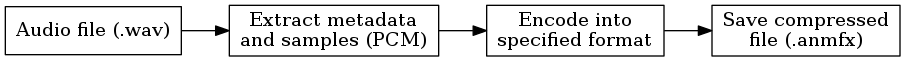
\includegraphics[width=\textwidth]{design_encoder.png}
\end{figure}

Next, each format's encoding process will be outlined (third step in the figure). If the audio file has multiple channels, this process is repeated on each channel separately.

\subsection{ANMF-RAW}
\begin{figure}[ht]
	\caption[ANMF-RAW Encoder]{The encoding scheme for ANMF-RAW.}
	\label{fig:encoding_nmf_raw}
	\centering
	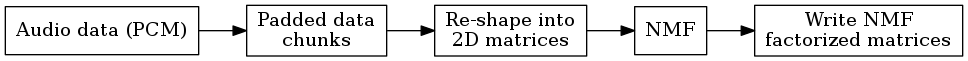
\includegraphics[width=\textwidth]{nmf_raw.png}
\end{figure}

ANMF-RAW works on the principle of applying NMF directly to the PCM audio samples $x_n$. However, the samples are initially an array of 16-bit signed integers, and as such, they need to be processed first before NMF can be used.

A chunk shape is specified to determine how many rows and columns each matrix will have before NMF. The sample array is then padded with zeros to ensure there are enough elements at the end of the array to ensure every matrix can have the same shape and number of elements. The amount of padding must be written to the output so that we know the length of the original array when decoding.

Once the array is padded, we iterate over the samples and split them into equal chunks of size $rows*columns$. This array is then "folded" to produce a matrix of the desired shape. We then obtain a matrix of signed integers, so in order to be able to use NMF, we first need to get rid of all the negative values. To do that, we increment each chunk by the absolute value of its smallest element, guaranteeing that the lowest value in the matrix is $\ge 0$.

Once we have this matrix, we proceed by applying NMF on it, obtaining the basis matrix $W$ and coefficient matrix $H$. Lastly, for each chunk, we write the value we incremented the matrix by, and the two decomposition matrices.

\begin{table}[htbp]\caption{ANMF-RAW data structure}
	\label{tab:anmf_raw_file}
	\centering
	\begin{tabular}{|c|c|l|}
		\hline
		Bytes (relative) & Data type & Description \\ \hline
		0-3 & uint32 & amount of zeroes used to pad the samples \\
		4-? & data\_chunk[] & NMF-compressed data chunks (refer to Table \ref{tab:anmf_raw_data}) \\
		\hline
	\end{tabular}
\end{table}

\begin{table}[htbp]\caption{ANMF-RAW structure of each data chunk}
	\label{tab:anmf_raw_data}
	\centering
	\begin{tabular}{|c|c|l|}
		\hline
		Bytes (relative) & Data type & Description \\ \hline
		0-7 & float64 & minimum value that the matrix was incremented by \\
		7-? & matrix(float32) & matrix $W$ \\
		?-? & matrix(float32) & matrix $H$ \\
		\hline
	\end{tabular}
\end{table}

\subsection{ANMF-MDCT}
\begin{figure}[ht]
	\caption[ANMF-MDCT Encoder]{The encoding scheme for ANMF-MDCT.}
	\label{fig:encoding_nmf_mdct}
	\centering
	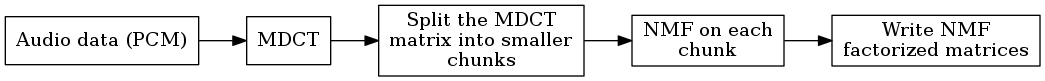
\includegraphics[width=\textwidth]{nmf_mdct.png}
\end{figure}

.. TODO ..

\subsection{ANMF-STFT}
\begin{figure}[ht]
	\caption[ANMF-STFT Encoder]{The encoding scheme for ANMF-STFT.}		\label{fig:encoding_nmf_stft}
	\centering
	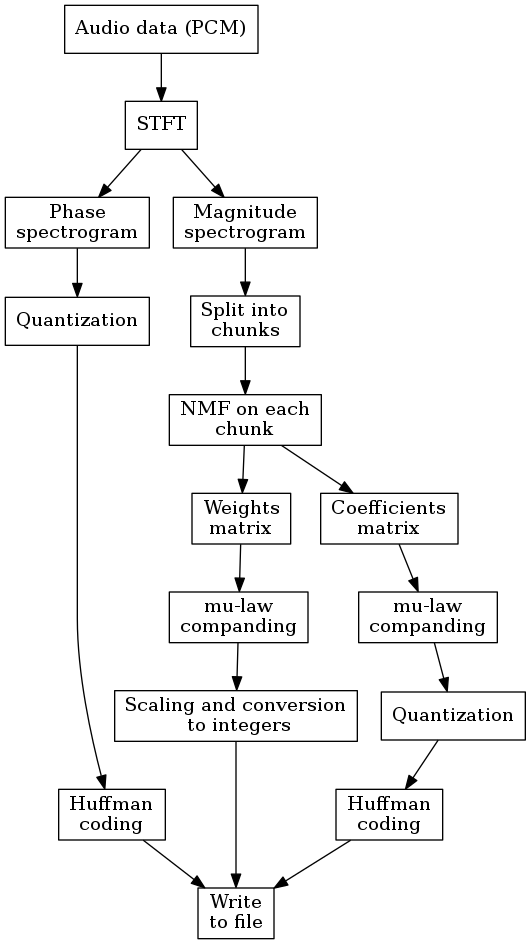
\includegraphics[width=0.6\textwidth]{nmf_stft.png}
\end{figure}

.. TODO ..

\section{Decoder}
Similar to the encoder, the decoder simply reverses the encoding process as seen in Figure \ref{fig:design_decoder}, and in each of the methods.

\begin{figure}[ht]
	\caption[Decoder overview]{A high level overview of the ANMF audio decoder.}
	\label{fig:design_decoder}
	\centering
	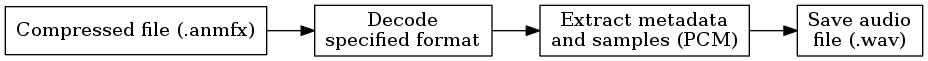
\includegraphics[width=\textwidth]{design_decoder.png}
\end{figure}

Next, each format's decoding process will be outlined.

\subsection{ANMF-RAW}
.. TODO ..

\subsection{ANMF-MDCT}
.. TODO ..

\subsection{ANMF-STFT}
.. TODO ..

mu-law quantization, non-uniform, formula in p128 wrong (missing sgn)\

- compressing MDCT

unusable, needs to be compressed consistently / losslessly

.. file structure ..

diagram for both time domain and frequency domain compression

